\chapter{Video Generation}\label{ch:results}

    In this chapter we combine the methods from the previous chapters. We also elaborate on some further preprocessing during the generation of videos. Finally we do our best to provide some results on paper.

    \section{Generating videos}
        
        Theoretically we can generate videos with each possible combination of extracted features and trained generators. The process is quite simple, the input song(s) are processed and melspectrograms are created. Depending on the chosen combination the melspectrograms are then used raw, encoded with the autoencoder, or processed through the CRNN. We then end up with 60 latent vectors per second of video, this information is used to create an image for each of those samples. From there we simply call ffmpeg to combine the images into a video, which is then combined with the input song.

    \section{Ensuring smooth transitions}
        
        Depending on the input song the resulting videos flickered and had very rapid and dramatic changes of images. As two very close latent vectors will produce a very similar image, the idea is to slow down our movement in the latent space. We realized this by implementing a gaussian smoothing with variable size. So depending on the song we can apply more or less smoothing.
        
        One might assume that the beginnning of change in an image should correlate with the beginning of change in sound. With this assumption we want to avoid smoothening future latent vectors into an image. Therefore we implemented a kernel that falls off very quickly in the direction of positive time, this results in a more smooth and slower movement through the latent space. For spikes in the song that only last a few frames, this smoothening will cause us to never reach the corresponding point within the latent space. Instead we move in the direction of that point but turn around / away before reaching it. More complex methods could be applied to shape our path through the latent space. For example, our path could be described using Bézier curve.

    \section{Results}

        Figure~\ref{fig:dcgan_samples} displays a collection of images that were generated with a DCGAN. We can observe that this particular model, which was using the raw melspectrograms as latent vector, manages to generate a wide variety of different flowers.

        \begin{figure}[ht]
            \centering
            \includegraphics[width=.94\textwidth]{images/fake_samples_not_cherry_picked}
            \caption[not used]
            {
                \textbf{A collection of images that were generated with a DCGAN. The latent vectors used to produce these images were randomly sampled from the music dataset.}
            }
            \label{fig:dcgan_samples}
        \end{figure}

        In figure~\ref{fig:video} we show a section of a melspectrogram and the images generated from that section. The images displayed here were produced without any smoothening techniques. Some images that showed little to no change have been omitted. A selection of example videos can be found here~\cite{examples}.

        \begin{figure}[ht!]
            \centering
            \fbox{
                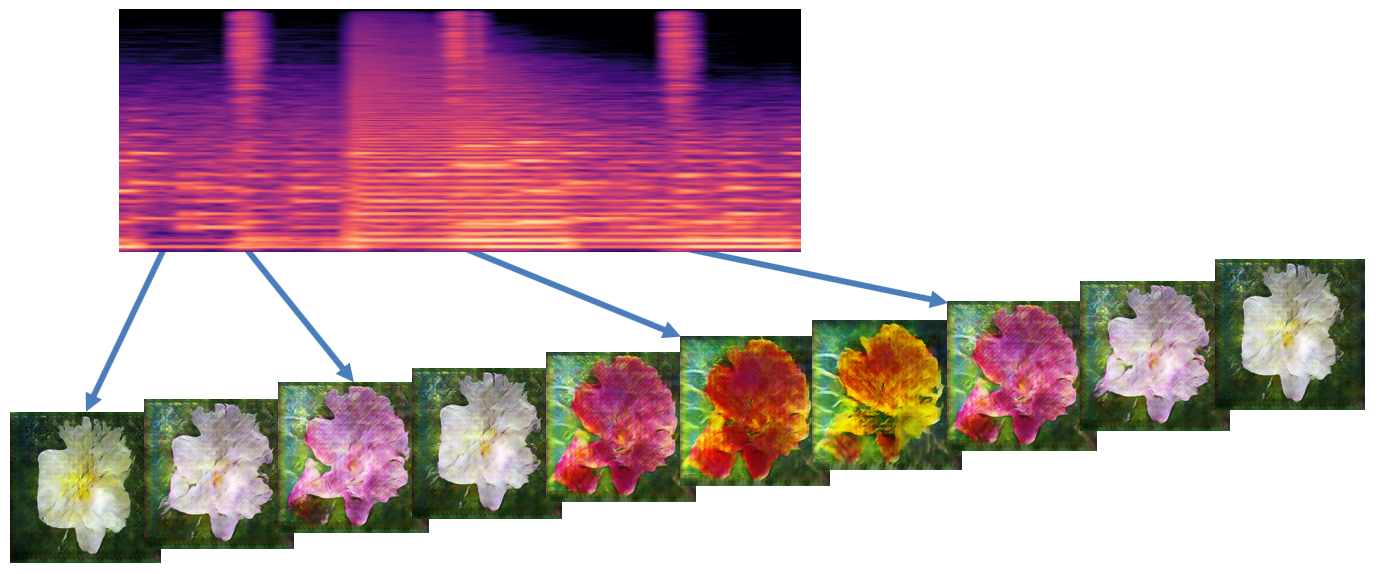
\includegraphics[width=.94\textwidth]{images/video_on_paper}
            }
            \caption[not used]
            {
                \textbf{An attempt at visualizing a resulting video on paper. We have connected the individual frames in the video with the underlying spectrogram. We can observe that similar sections in the melspectrogram produce very similar flower images.}
            }
            \label{fig:video}
        \end{figure}

        \section{Visualizing your own music}
            If the reader of this report would like to generate a visualization of a music track of his likings, he can download a compact version of a pretrained generator from our Google Drive~\cite{visualizer}. After extracting the zip file, one can place their desired mp3 file in the $song\_in$ folder and execute either \textit{start\_cuda.sh} or \textit{start\_cpu.sh}, if your device does not support cuda (warning, this can take very long). We currently only support the video generation directly from the mel spectrograms due to the mixed results of the other approaches. The script will then automatically calculate the mel spectrogram of the given song, apply a Gaussian smoothing over the time steps, feed the vectors to the pretrained generator and afterwords compile the images to a single video with the song added as the audio track. The resulting video will appear in the $song\_out$ folder adjacent to the $song\_in$ folder after everything is completed. If you would like to experiment with the smoothing, you can either change the kernel size with the \textit{smooth\_count} parameter, or disable smoothing entirely by removing the \textit{smooth} parameter from the respective bash scripts. The whole procedure requires a variety of python packages, as well as ffmpeg installed on the system. We cannot guarantee that every genre will deliver satisfying results, an average metal song seemed to throw off the results quite a bit, but maybe you have some fun with the generators. Also the names of the output files might be a bit cryptic.